\newcommand{\HRule}{\rule{\linewidth}{0.5mm}}
\newcommand{\TODO}[1]{\textcolor{red}{TODO: #1}}
\newcommand{\cosmin}[1]{\textcolor{green}{Cosmin: #1}}

\newcommand{\mychapter}[2]{\chapter{#1}\label{#2}}
\newcommand{\mysection}[2]{\section{#1}\label{#2}}
\newcommand{\mysubsection}[2]{\subsection{#1}\label{#2}}

%\begin{figure}[h!]
%\begin{center}
%  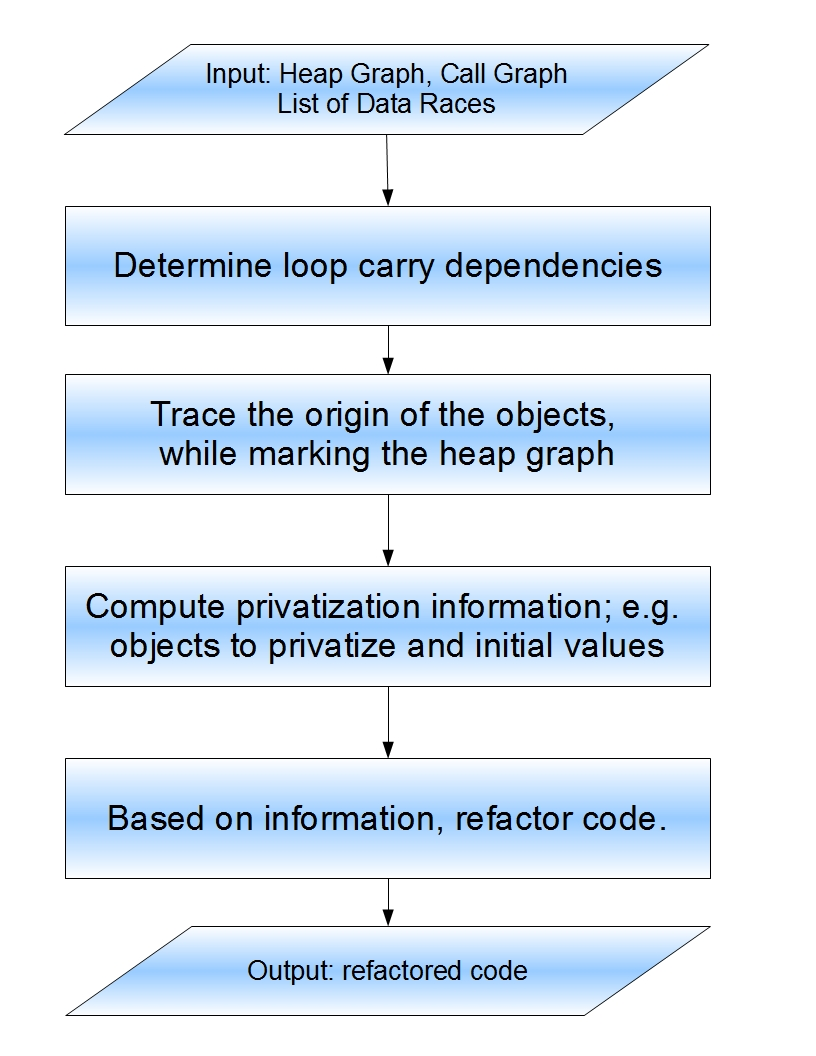
\includegraphics[width=7cm]{algo}
%  \caption{Flow chart coarsely describing the tool}
%  \label{algo}
%\end{center}
%\end{figure}

\newcommand{\myfigure}[5]{
\begin{figure}[h!]
	\begin{center}
		\includegraphics[width=#5]{#1}
		\label{#2}
		\caption[#3]{#4}
	\end{center}
\end{figure}
}

\newcommand{\lcd}{\emph{loop-carried dependency}}
\newcommand{\lcds}{\emph{loop-carried dependencies}}

\newcommand{\slcd}{\emph{loop-carried dependency }}
\newcommand{\slcds}{\emph{loop-carried dependencies }}
